\section{APLICACION} 
		
\begin{enumerate}[1.]

	\item Aplicaciones BI :
\\
\\
 Una de las claras tendencias en el mercado Business Intelligence es la mayor importancia que los clientes otorgan a visualizar la informaci\'on de una manera sencilla, \'agil y potente. Todo a la vez.
\\
\\
- La entrega de informaci\'on contin\'ua siendo el foco central de la mayor\'ia de los proyectos de BI en la actualidad, pero vemos una creciente demanda de herramientas que permitan un an\'alisis más fácil e intuitivo para descubrir nuevas perspectivas. (Gartner, 2010)
\\
\\
-Pr\'oxima generaci\'on de aplicaciones de Business Intelligence pretenden ir más all\'a de la provisi\'on de informaci\'n en gr\'aficos circulares y estad\'isticos, para proporcionar representaciones m\'as visuales e intuitivas de datos y tendencias. (IDG)
\\
\\
- Herramientas como la visualizaci\'on de datos (en formatos que van m\'as all\'a de las simples im\'agenes est\'aticas) permiten presentar informaci\'on de forma clara y eficaz. La visualizaci\'on de datos ha estado directamente relacionada con las tecnolog\'ias de BI desde su origen y la b\'usqueda continuada de presentaciones m\'as eficaces e interactivas a trav\'es de la visualizaci\'on ser\'a uno de los objetivos de las soluciones anal\'iticas de los pr\'oximos años. (Federico Navarro Cabrera, de IBM)
\\
\\
Hasta hace muy poco, el Business Intelligence era una manera m\'as o menos sencilla de generar informes, listados, an\'alisis, o "reportes"(¡que horrible palabra!)... Al final, todo era m\'as o menos lo mismo... Informes tabulares, con filas y columnas llenas de n\'umeros, y alg\'un gr\'afico. Las herramientas m\'as avanzadas permit\'ian añadir alertas semaf\'oricas, parametrizar el informe, o alg\'un tipo de navegaci\'on OLAP (que raramente se utilizaba)... Este tipo de soluciones ya han llegado a su madurez, y existe muy poca diferencia entre la oferta de los diferentes proveedores..
\\
Sin embargo, esta manera tradicional de acceder a la informaci\'on resulta insuficiente (e ineficiente), y cada vez m\'as las organizaciones buscan maneras de proporcionar a sus usuarios soluciones para acceder, analizar y comprender la informaci\'on corporativa de una manera m\'as sencilla, din\'amica, visual e intuitiva. El cambio es realmente profundo, y supone una renovaci\'on completa en las "interfases de usuario"...
\\
Estoy hablando de soluciones tipo QlikView, Tableau o, por supuesto, Bingo Intelligence... que buscan la mayor usabilidad para el usuario final, y ofrecen soluciones Business Intelligence muy interactivas y visuales... Os dejo algunos pantallazos de Qlickview y Tableau.

\end{enumerate}

\begin{center}
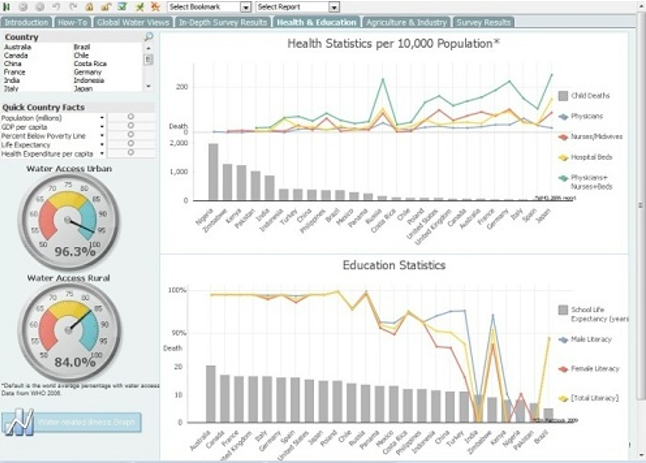
\includegraphics[scale=0.60]{./Imagenes/img1.png}
\end{center}

\begin{center}
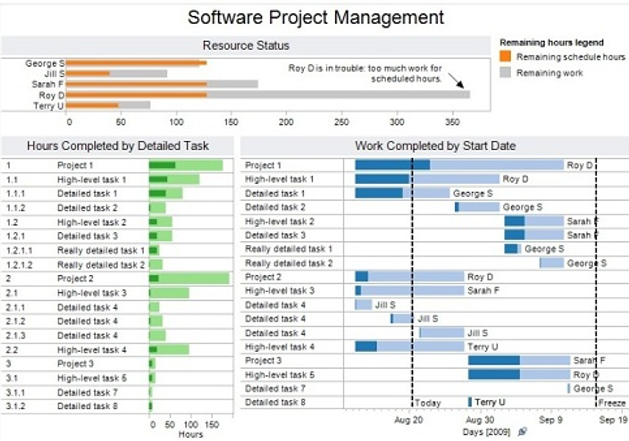
\includegraphics[scale=0.60]{./Imagenes/img2.png}
\end{center}

\begin{center}
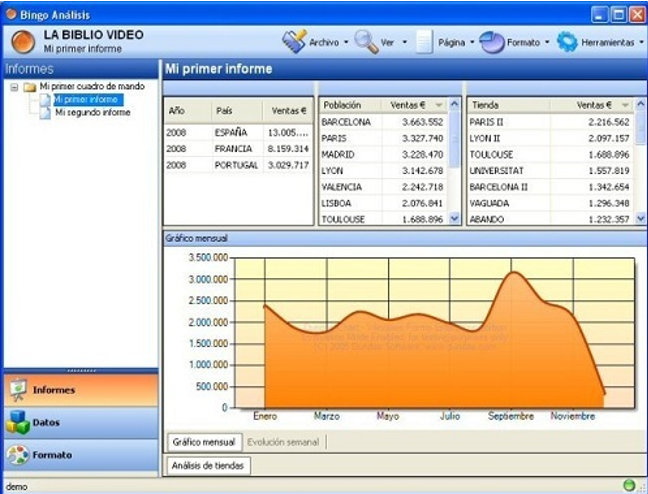
\includegraphics[scale=0.60]{./Imagenes/img3.png}
\end{center}

\begin{center}
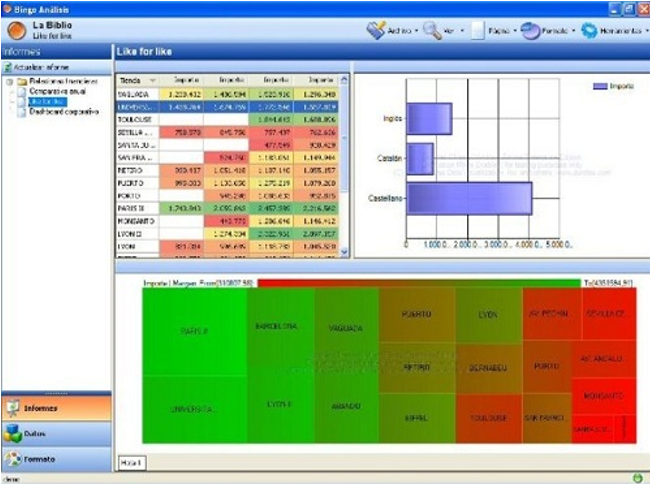
\includegraphics[scale=0.60]{./Imagenes/img4.png}
\end{center}

\begin{enumerate}[2.]

	\item Aplicaciones BA :
\\
\\
Empecemos con un ejemplo de su aplicaci\'on una cafeter\'ia quiere elegir la ubicaci\'on de un nuevo local en Lima. Antes de tomar esta decisi\'on tienen que estar muy seguros sobre la ubicaci\'on de este, porque una vez creado el local, revertir la situaci\'on seria muy costoso. Los usuarios de internet podr\'ian proporcionar informaci\'on sobre su lugar de residencia y sobre posibles locaciones en las cuales les gustar\'ia que el local este ubicado para poder asistir, tambi\'en se puede encontrar informaci\'on de zonas en las que no est\'e presente una empresa de este rubro para poder abarcarla. Lo que hace BA, es recuperar toda esta informaci\'on para ayudar a la empresa a definir sus planes y poder explicar el porqué de la elecci\'on de su nueva locaci\'on. Confiar en este tipo de datos que proporciona BA reduce el riesgo de tomar una decisi\'on desinformada y err\'onea.
\\
\\
Enfocado al marketing podemos decir que las empresas usan el BA para sacar ventaja a la competencia, ya que se anticipan a las nuevas necesidades de cliente. Se pueden relevar nuevas tendencias de consumo o uso de los productos con el uso del BA.
\\
\\
El poder de transformaci\'on de los datos es realmente grande, sin embargo, el poder no est\'a en los datos por s\'i solo, sino tambi\'en a medida que se pulen a trav\'es de an\'alisis. Aunque la anal\'itica se ha convertido en parte de un lenguaje diario, definimos el BA como el proceso de descubrimiento de conocimiento para la acci\'on y la creaci\'on de nuevas oportunidades de negocio a partir de esos descubrimientos. La lecci\'on principal es ligar fuertemente en BA a los negocios. Para ello, se tiene que crear intersecciones seguras y productivas con el personal que se encarga del análisis y los decisores estrat\'egicos.


\end{enumerate}

